\section{Problem 3}

This problem will address the transmission line of figure \ref{p3:line3}. The objective of this problem is to validate the results of the S-parameters. First of all the calculations will consider terminations of $Z_S = Z_L = Z_0 = 50 \Omega$, line characteristic impedance of $Z=75 \Omega$ and frequency of $1 GHz$. Then after the frequency will seep between $500 MHz$ and $1.5 GHz$. 

\begin{figure}[H] 
\centering
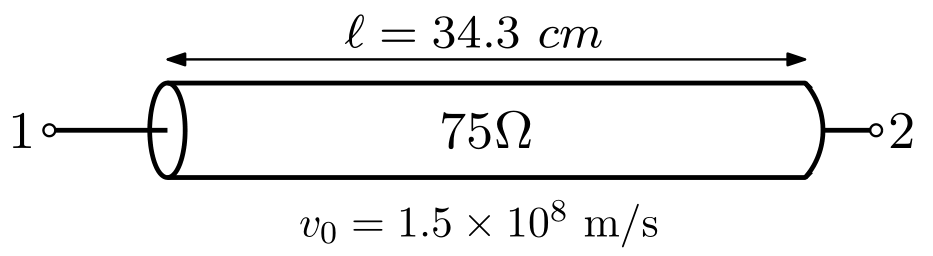
\includegraphics[width=9cm]{images/line3.png}
\caption{Transmission line for problem 3.}
\label{p3:line3} 
\end{figure}

\subsection{Theoretical values for S-parameters}

Once the circuit is symmetrical, the input impedance seen in each port is the same and computed by the equation \ref{p3:zin}

\begin{equation} \label{p3:zin}
    Z_{in} = Z \frac{Z_0 + jZ \, tg(\beta l)}{Z + jZ_0 \, tg(\beta l)} 
\end{equation}

Where $\beta = 2\pi/\lambda$ and $\lambda = v_0/f$, resulting in $Z_{in} = 107.52 \angle -10.38 ^{\circ} \Omega$.

So both the reflection coefficients and, therefore the coefficients of the S matrix main diagonal are:

\begin{equation} \label{p3:s11s22}
    |s_{11}| = |s_{22}| = \left|\frac{Z_{in}-Z_0}{Z_{in}+Z_0}\right| = 0.376 \; \; or \; \; -8.49 dB
\end{equation}

Considering a lossless line, the output power will be equal to the input power. But the input power is the total power available at the source subtracted the reflection losses, resulting in $P_{out} = P_{in} = P_{av,s} - P_r$. Since the reflection losses are a portion of the available power scaled by the reflection coefficient: $P_r = |s_{11}|^2 P_{av,s}$, the expression for the output power can be rewritten as: $P_{out} = P_{av,s} (1-|s_{11}|^2)$; resulting in a power transmission coefficient of $|s_{21}|^2 = 1-|s_{11}|^2$. The same can be deducted from the second port point of view resulting in $|s_{12}|^2 = 1-|s_{22}|^2$. This results in the coefficients for the S matrix secondary diagonal at the equation \ref{p3:s21s12}.

\begin{equation} \label{p3:s21s12}
    s_{21} = s_{12} = \sqrt{1-|s_{11}|^2} = \sqrt{1-|s_{22}|^2} = 0.926 \; \; or \; \; -0.667 dB 
\end{equation}

It is good to remember that the equations $|s_{11}|^2 + |s_{21}|^2 = 1$ and $|s_{22}|^2 + |s_{22}|^2 = 1$ are true in a lossless condition only.

\subsection{Simulated values for S-parameters}

Using the ADS to simulate the previous circuit in a S-parameters simulation, the curves for the magnitude of all matrix S coefficients as seen in figure \ref{p3:sparams} in a range of $500 MHz$ to $1.5 GHz$.

\begin{figure}[H] 
\centering
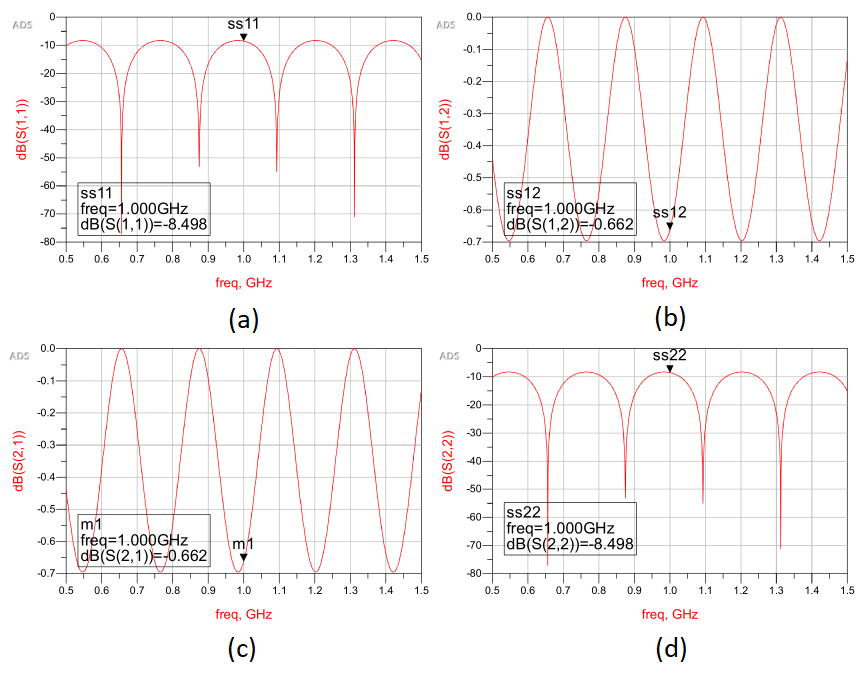
\includegraphics[width=15cm]{images/sparamsp3.png}
\caption{Problem 3 circuit S-parameters: (a) $s_{11}$, (b) $s_{12}$, (c) $s_{21}$ and (d) $s_{22}$.}
\label{p3:sparams} 
\end{figure}

Observing the markers in figure \ref{p3:sparams} show the results for each one of the S-parameters at $1GHz$ in dB and they agree with the values obtained is the previous calculations expressed in the equations \ref{p3:s11s22} and \ref{p3:s21s12}.

Regarding to the relation $|s_{11}|^2 + |s_{21}|^2 = 1$ explained before, it can be obtained in the ADS simulation and its veracity does not depend on the frequency, as seen in figure \ref{p3:unit}.

\begin{figure}[H] 
\centering
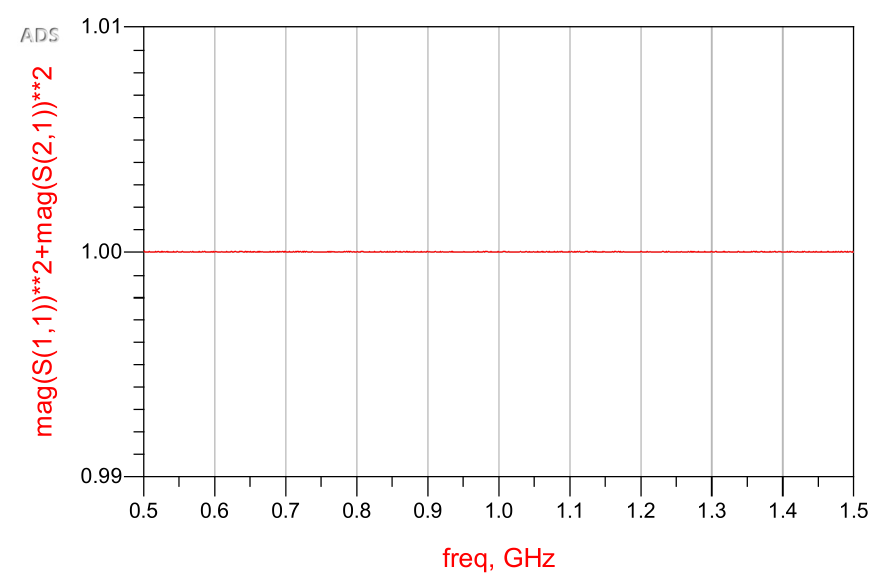
\includegraphics[width=9cm]{images/unit.png}
\caption{$|s_{11}|^2 + |s_{21}|^2 = 1$ relation in ADS.}
\label{p3:unit} 
\end{figure}
